% ============================= Info ============================= %

% Applied Machine Learning Systems ELEC0132 Assignment
% Due 11:59pm, 07 Jan 2019

% 6 double-column single-spaced pages 
% Plus up to 4 pages of supplementary material 
% (methodology clarification, additional results, other tests, etc.)

% Include hidden link to code in public repo (Dropbox, Drive, etc.)

\iffalse
Assignment tasks:
	- Detection and removal of noisy images
	- Training, validation and testing subsets division
	- Train ML models to perform
		Binary tasks
			1. Emotion recognition (smile/!smile)
			2. Age identification (young/old)
			3. Glasses detection (with/without)
			4. Human detection (real/avatar)
		Multiclass tasks
			5. Hair colour recognition (ginger, blond, brown, grey, black, bald)
\fi

% =========================== Packages =========================== %
\documentclass[conference]{IEEEtran}
\usepackage{amsmath, graphicx, multicol, cite}
\usepackage{color}
\usepackage{listings}% code
%\usepackage{refcheck}
\lstset{escapeinside={<@}{@>}}

% ============================= Title ============================= %
\begin{document}

\title{Applied Machine Learning\\
 Systems ELEC0132 Assignment}
\author{\large Maryam Habibollahi\\ \textit{Department of Electronic and Electrical Engineering}\\ \textit{University College London}\\ zceemha@ucl.ac.uk}
\date{November 2018}
\maketitle

\setcounter{page}{1} \pagenumbering{arabic}

% ============================ Abstract =========================== %
\begin{center} \large \textbf{Abstract} \end{center}
\textit{Brief overview of the methodology/results presented.}\\

% ========================== Introduction ========================== %
\section{Introduction} \label{s-intro}

% The problem statement.\\

% Why face recognition, why classification? (applications, need, PROBLEM!)
The perception of visual information is a key element of human communication, particularly those from the face. The features and characteristics of an individual's face can provide information of their identity, emotion, and intent, with potential applications in access and security, law enforcement, marketing, and banking. Researchers in the fields of computer vision have been developing technological breakthroughs %?
in the implementation of face recognition using machine learning tools and techniques over the past decades.
% Problem
The image variations of real-world scenarios such as illumination, pose, expressions, and occlusions 
have required more complex methods in need of preprocessing techniques to prepare images for training and classification. 
% ^ FIX THIS!!

% Assignment + dataset description:
% summarising data (content, size, format, etc.) and describing any \textit{data preprocessing} applied.\\
This assignment aims to train machine learning models and perform binary and multiclass classification on a large dataset of 5000 Portable Network Graphic (PNG) image files consisting of pre-processed subsets from the \textbf{CelebFaces Attributes Dataset (CelebA)}, a celebrity image dataset  % CITE!
%(S. Yang, P. Luo, C. C. Loy, and X. Tang, "From facial parts responses to face detection: A Deep Learning Approach", in IEEE International Conference on Computer Vision (ICCV), 2015
, and the \textbf{Cartoon Set}, an image dataset of random cartoons/avatarts % CITE!
%(source: https://google.github.io/cartoonset/)
, as well as a number of noisy images (mainly of natural backgrounds) to be detected and removed from the training data, which generally constitues 80\% of the entire dataset.
All images are labelled with hair colour, whether the subject is wearing glasses, is smiliing, and is classified as human.

In order to train a suitable model for the required classification tasks, several preprocessing methods were taken into consideration to provide appropriate features for the process; for instance, facial landmarks were extracted upon face detection to train models using supervised learning algorithms such as Support Vector Machines (SVM) or  Multi-Layer Perceptor (MLP) models based on the extracted facial landmarks.
% ^ ref to additional material for picture of landmarks and more explanation on HOGm Haar-cascade, etc.
A comparative analysis of the performance of each method with respect to the labaled noisy images %(where all labels are defined as -1) 
facilitated the selection of the most appropriate feature extraction method for the given dataset.

Prior to feature extraction, various preprocessing techniques were carried out on the images to improve both the performance and the processing power during the later stages of the extraction, training and classification procedures. 
% ^ pre-pre-processing? or data preparation _for_ preprocessing?
Some of the techniques include colour space transformation, capable of significantly reducing processing complexity, gamma correction (power-law equalisation), a non-linear function used to normalise illumination by raising the input value to the power $\gamma$, and mean normalisation.%, etc.
% ^ Elaborate + Equations

The original dataset was otherwise rescaled and augmented to avoid overfitting for alternative models more specifically used for visual recognition tasks, such as Convolutional Neural Networks (CNN), where the noisy images of the training and validation data are removed using the results of the optimum face detector method with the maximum accuracy. % Duh

% ======================= Proposed algorithms ====================== %
\section{Proposed algorithms} \label{s-algorithms}

% Algorithmic approach used to solve the problem.\\
% Explain rationale behind choices, i.e. detail your \textit{reasons for selecting a particular model}.\\

% Feature extraction methods 
A major step of the extraction of facial information for various classification tasks such as age, gender, emotion, and other attributes apparent on the face is to localise the fiducial facial key points \cite{landmark_lit}. The landmarks provide a set of $x$ and $y$ coordinates that either describe the specific points that describe a unique location of a particular component, or lay out the contours connecting those points, such as those shown in Figure \ref{fig: landmarks}.
Several algorithms have been developed to achieve this purpose, namely the Haar cascade classifier, the first real-time face detector proposed in 2001, the Histogram of Oriented Gradients feature with a linear classifier, and various Deep Learning-based detectors, which are significantly more accurate than the former two methods, though at a cost of higher complexity.
% TODO: How does the HOG work?

\begin{figure} [h] % Landmarks
  \centering
    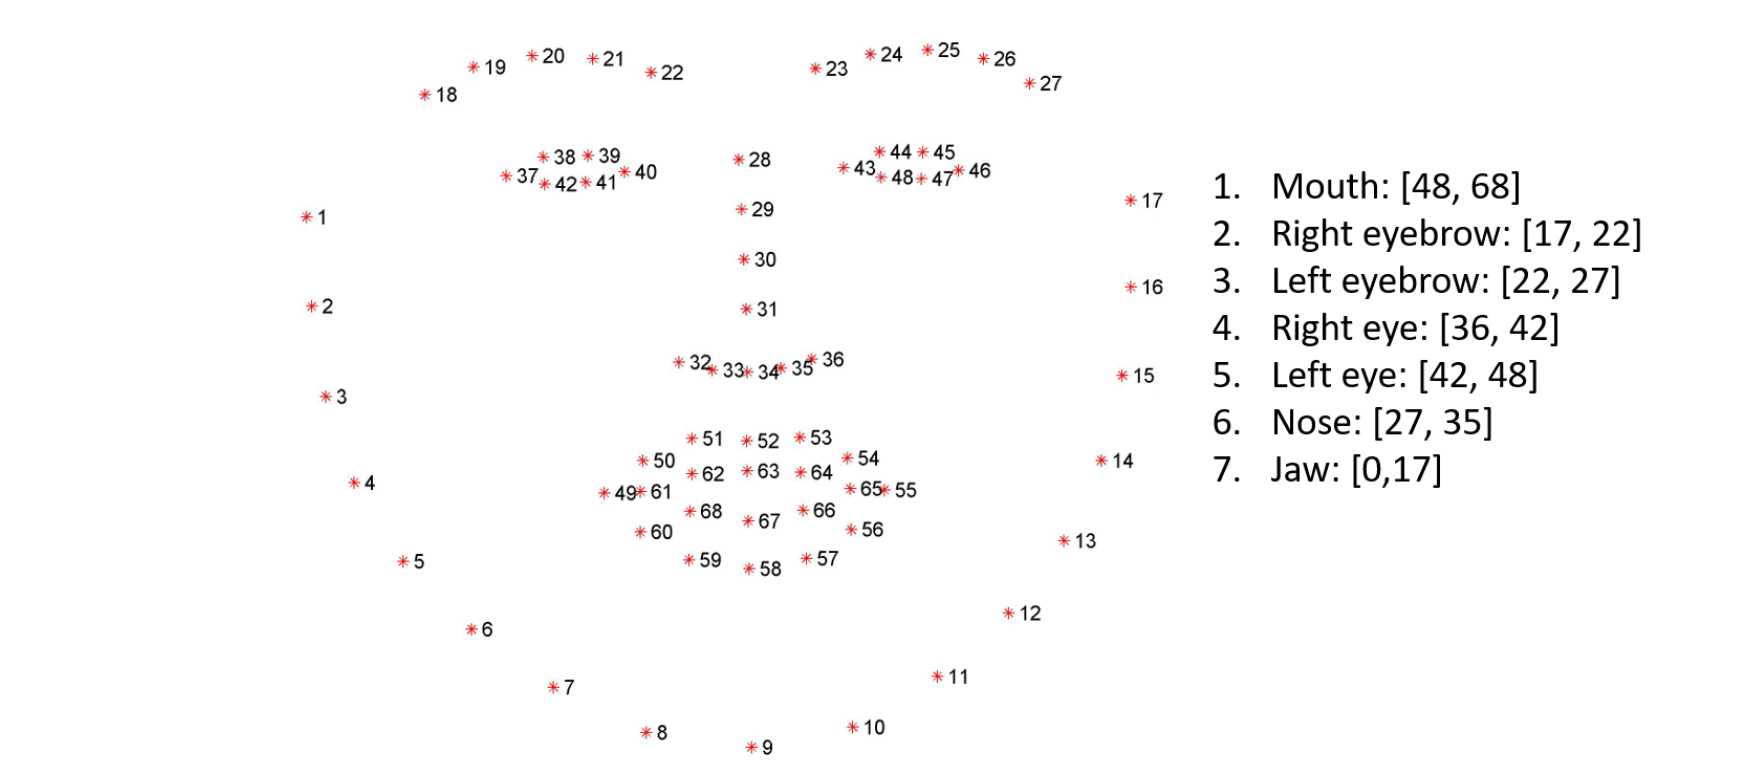
\includegraphics[width=0.5\textwidth]{graphs/landmarks} 
    \caption{Face shape defined by 68 landmarks}
    \label{fig: landmarks}
\end{figure}

The relative balance between the expected accuracy and complexity of a HoG detector with respect to the Haar casccade and Deep Learning options makes it preferable for this dataset. Nonetheless, a comparative analysis was perfomed by recording the accuracy and training time of each detector as a measure of performance and complexity.

% SVM model
Classification of the binary tasks was performed using the landmark features to train models with supervised learning algorithms, namely Support-Vector Machines (SVM), which are capable of linearly separating classes in a high-dimensional space through the implementation of different kernel functions. 
% Gradient descent
The hyperplane which isolates one class from another can be refined via gradient descent, an iterative optimisation algorithm, such as that shown in Equation \ref{eq: GD}, which represents the gradient in linear regression for a model of n data points and m features. This technique is used to minimise a parameter called the cost function, which represents an attribute of the error in the response, such as the squared sum of residuals.
% TODO: Hyperparameter selection

\begin{equation}
\theta_{j+1} = \theta_j - \frac{\alpha}{n} \sum_{i=1}^n \bigg[\sum_{k=1}^m \theta_k x_k^{(i)} - y^{(i)} \bigg] x_j^{(i)} 
\label{eq: GD}
\end{equation}

% MLP model
Higher-complexity models based on artificial neural networks that are capable of providing higher accuracies were also implemented using the features extracted. A Multi-Layer Perceptron (MLP) model, which carries out the training using Backpropagation, an efficient method that computes the partial derivates in gradient descent, was therefore selected for the binary tasks. The derivatives are calculated from each layer's error term, $\delta_i^l$, which is computed using Equation \ref{eq: backprop}, for $a^{(l)}$ representing the activation vector of layer $l$, resulting in the output $z^{(l)} = \theta^{(l)} a^{(l)}$ for that layer.
% TODO: Hyperparameter selection

\begin{equation}
\delta^{(l)} = \big(\theta^{(l)}\big)^T \delta^{(l+1)}.g'(z^{(l)})
\label{eq: backprop}
\end{equation}

% CNN model
Despite the minimised processing requirement when the landmark features are used, they pose limitations to classification tasks less reliant on the key component locations, and requiring important information ommited from the images such as colour. Thus, for the final task of detecting hair colour, a more commonly-used classifier for image processing with multilayer neural networks called Convolutional Neural Networks (CNN) was implemented on a LeNet architecture. The popularity of CNNs in image classification is primarily due to the 3D volumes of neurons, resuling in connectivities of small regions between layers (known as the receptive field), which can result in a lower complexity than the traditional neural networks, while taking advantage of 3-dimensional images. 
% LeNet architectures
The LeNet architecture is a small yet powerful tool for image classification using CNN. Primarily used for Optical Character Recognition (OCR), LeNet implements a 7-level convolutional network composed of convolutional layers, (ReLU) activation and pooling layers, as illustrated in Figure \ref{fig: LeNet}.

\begin{figure} [h] % LeNet architecture from LeCun
  \centering
    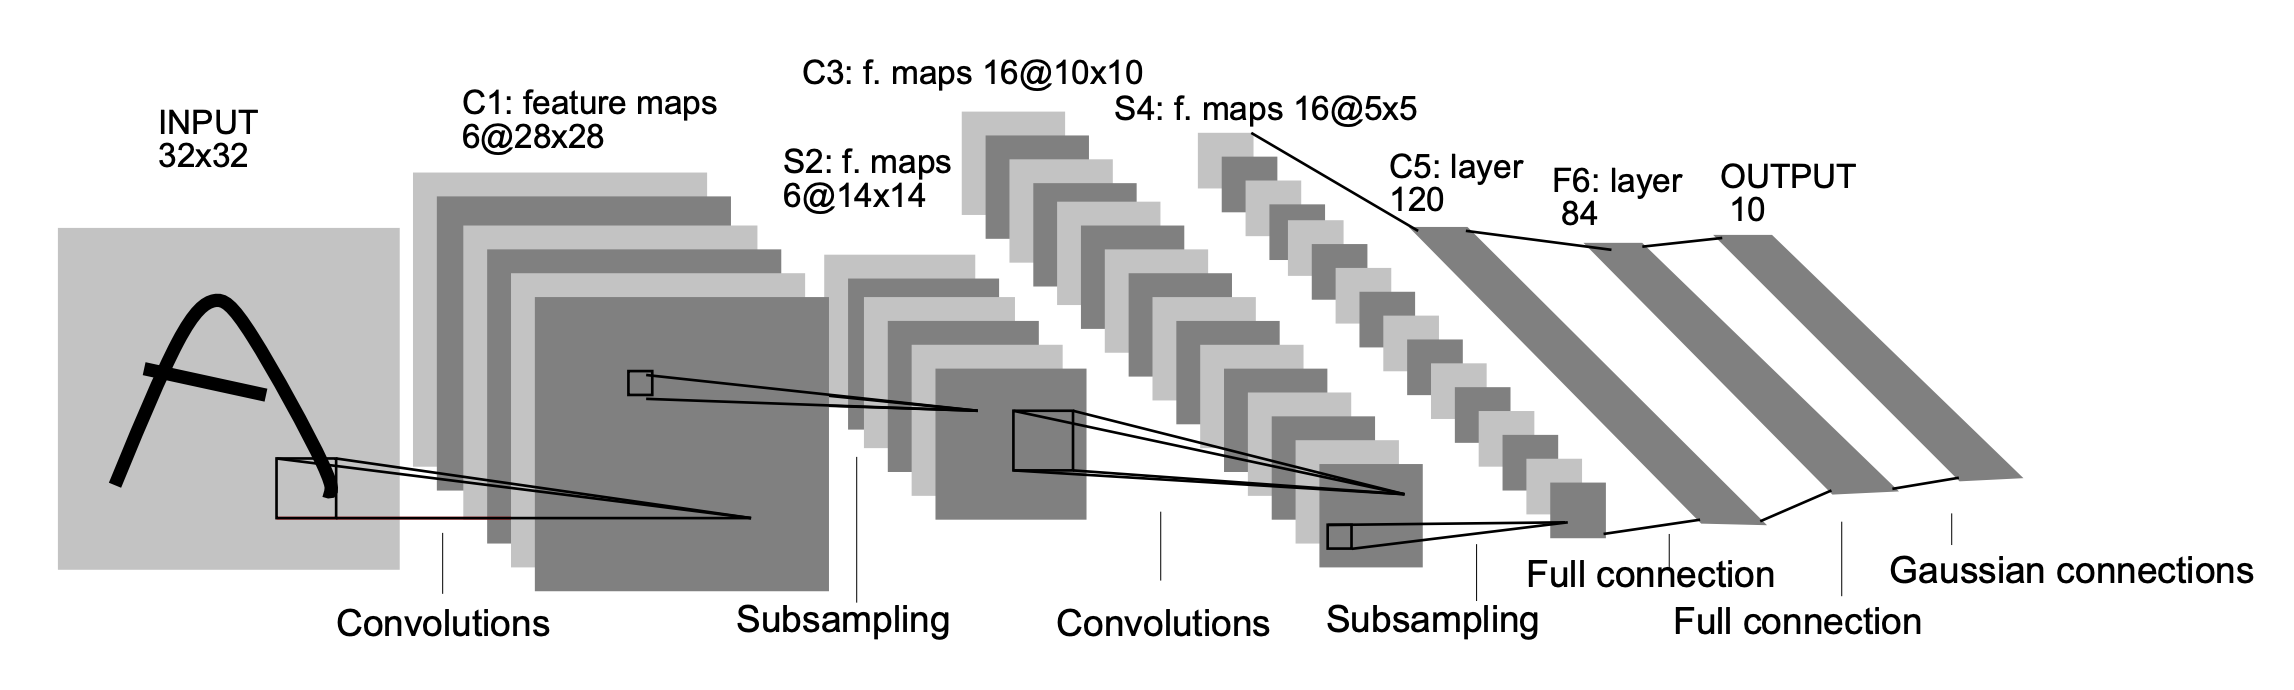
\includegraphics[width=0.5\textwidth]{graphs/LeNet} 
    \caption{Architecture of LeNet-5 by LeCun et al. \cite{LeCun}}
    \label{fig: LeNet}
\end{figure}

% Expected performance - overfitting
Increasing the number of layers in a neural network is often believed to provide a better model, given the higher complexity. However, a model can be easily overfit to the training set if the parameters follow the data too closely.
In order to obtain a more generalised model of the data, cross-validation was selected to perform out-of-sample testing on the dataset.
% TODO: Explain cross-validation

% ========================= Implementation ======================== %
\section{Implementation} \label{s-implement}

% Provide name and use of \textit{external libraries} and explain how \textit{model parameters} were selected.\\

% Preprocessing
Two of the main Python libraries 

% scikit-learn -> svm, neural networks, etc.
The 

% cross-validation methods on various parameter values

Thorough discussion on the training convergence and stopping criterion (use learning curves graphs).\\

% ======================= Experimental results ====================== %
\section{Experimental result} \label{s-exp-res}

Describe and discuss results, compare to other approaches in literature or variations of ML solutions.\\

Include \textit{accuracy prediction scores on a separate test dataset, provided by the module organisers, but not used during training and validation}.\\

% ========================== Conclusion ========================== %
\section{Conclusion} \label{s-concl}

Summaries all findings and suggest direction for future improvement.\\

% ========================= Related work ========================== %
\section{Related Work} \label{s-rel-work}

Summarise latest reserach on the topic, discussing merits/disadvantages of diff approaches.\\

% ========================== References ========================== %

\bibliographystyle{IEEEtran}
\bibliography{/Users/MaryamH/Documents/BibTex/library}

\end{document}
